\documentclass[../240513_msquare_shor.tex]{subfiles}

\begin{document}

\subsection{Quantum Computing}
\begin{frame}{Quantum Computing}
    \begin{block}{Quantum State}
        A \textit{quantum state} is a
        unit-length vector in an \(N\)-dimensional complex vector space.
    \end{block}
    \pause
    \begin{figure}
        \centering
        
\includegraphics[width=.7\textwidth]{images/observe.png}
    \end{figure}
    \begin{block}{Observation}
        If \(v = \sum_{i=0}^{N-1} a_i \vert b_i \rang\)
        where \(\vert b_i \rang\)'s are basis vectors (also called \textit{pure states}),
        \(v\)를 ``관측''하면 \(\vert b_i \rang\) 중 하나를 보게 되는데,
        \(\vert b_i \rang\)을 관측할 확률은 각각 \(|a_i|^2\)임.
    \end{block}
\end{frame}

\begin{frame}{Quantum Fourier Transform}
    \begin{figure}
        \centering
        
\includegraphics[width=.7\textwidth]{images/fourier.jpg}
    \end{figure}
\end{frame}

\begin{frame}{Quantum Fourier Transform}
    \begin{center}
        \fbox{\(\omega = e^{2\pi i / N}\)}
    \end{center}
    \begin{block}{Quantum Fourier Transform}
        Quantum Fourier transform은 basis vector \(\vert b_i \rangle\)를
        \[
            | b_i \rang \longmapsto
            \frac{1}{\sqrt{N}} \sum_{j = 0}^{N-1} \omega^{ij} | b_j \rang
        \]
        로 보내는 linear map이다.
    \end{block}
    \pause
    \begin{exampleblock}{Blackbox}
        임의의 \(N\)-dimensional quantum state에 대한
        QFT를 \(O((\log N)^2)\) 시간 안에 계산 가능하다.
    \end{exampleblock}
\end{frame}

\subsection{Calculating the Order}
\begin{frame}{Calculating the Order: Overview}
    \begin{figure}
        \center
        
\includegraphics[width=.7\linewidth]{images/saving_order.png}
    \end{figure}
\end{frame}

\begin{frame}{Calculating the Order: Overview}
    \begin{block}{Calculating the Order}
        목표: Fixed \(x, n\)에 대해 \(\ord_n x\)를 찾기.
        \begin{enumerate}
            \ii
            \(N = 2^\ell\), \(n^2 < N < 2n^2\)인 \(N\) 찾기. (Easy!)
            \ii
            \((N + n)\)-dimensional quantum state를 다음으로 초기화.
            \[
                \frac{1}{\sqrt{N}} \sum_{i=0}^{N-1} | i, x^i \mod n \rang
            \]
            (Basis vector들을 \(|a, b \rang\), \(0 \le a < N\), \(0 \le b < n\) 꼴로 나타냄.)
            \ii
            위 quantum state의 first register에 대해 quantum fourier transform 적용.
            (디테일은 뒤에서)
            \ii
            관찰. \(| j, x^i \mod n \rang\)을 관찰했다고 하자.
            \ii
            운이 좋으면 \(j/N\)의 convergent (continued fraction)의 분모 중
            \(\ord_n x\)가 등장함! (\(\text{확률} \in \Omega(1/\log \ell)\))
        \end{enumerate}
    \end{block}
\end{frame}

\begin{frame}{Calculating the Order: Initialization}
    \begin{exampleblock}{Initialization Step (2)}
        \begin{enumerate}
            \ii
            Quantum state를
            \[
                \frac{1}{\sqrt{N}}\sum_{i=0}^{N-1} | i, 0 \rang
            \]
            으로 초기화
            \pause
            \ii
            \(| i, 0 \rang \mapsto |i, x^i \mod n \rang\)으로 보내는 linear map
            을 계산.\footnotemark 
            \[
                \frac{1}{\sqrt{N}}\sum_{i=0}^{N-1} | i, x^i \mod n \rang
            \]
            \footnotetext{time complexity: \(O(\ell^2 \log \ell)\)}
        \end{enumerate}
    \end{exampleblock}
\end{frame}

\begin{frame}{Calculating the Order: QFT}
    \begin{exampleblock}{Quantum Fourier Transform (3)}
        \[
            \frac{1}{\sqrt{N}}\sum_{i=0}^{N-1} | i, x^i \mod n \rang
        \]
        의 QFT를 \(O(\ell^2)\) blackbox algorithm으로 계산:
        \pause
        \[
            \frac{1}{N}\sum_{i=0}^{N-1}\sum_{j=0}^{N-1} \omega^{ij} | j, x^i \mod n \rang
        \]
    \end{exampleblock}
\end{frame}

\begin{frame}{Calculating the Order: Observation}
    \[
        \frac{1}{N}\sum_{i=0}^{N-1}\sum_{j=0}^{N-1} \omega^{ij} | j, x^i \mod n \rang
    \]
    \begin{exampleblock}{Observation (3)}
        Basis vector \(| j, x^i \mod n \rang\) (\(0 \le j < N\), \(0 \le i < \ord_n x\))을 관측할 확률은?
        \pause
        \begin{center}
            \fbox{Note that \(x^i \equiv x^{i + r} \equiv x^{i + 2r} \equiv \cdots \pmod{n}\) where \(r = \ord_n x\)!}
        \end{center}
        \pause
        \[
            \left| \frac{1}{N} \sum_{b=0}^{m-1} \omega^{rjb} \right|^2
            = \frac{1}{N^2} \cdot \frac{\sin^2(\pi m rj / N)}{\sin^2(\pi rj / N)}
        \]
        where \(m = \lfloor (N - i - 1) / r \rfloor + 1 \approx N / r\).
    \end{exampleblock}
\end{frame}

\begin{frame}{Calculating the Order: Observation}
    \[
        \Pr\big[\text{observing}~ | j, x^i \mod n \rang\big]
        = \frac{1}{N^2} \cdot \frac{\sin^2(\pi m rj / N)}{\sin^2(\pi rj / N)}
    \]
    \begin{figure}
        \centering
        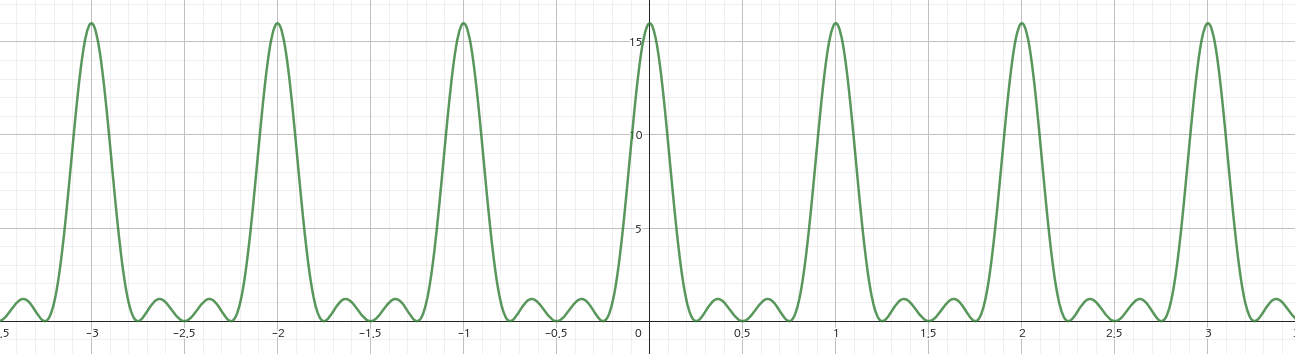
\includegraphics[width=\textwidth]{images/probability.png}
    \end{figure}
    \begin{center}
        \pause
        \(\dfrac{rj}{N}\)이 정수에 가까운 \(j\)를 관찰할 확률이 크다! \\
        \pause
        즉, \(\dfrac{j}{N}\)이 \(r\)을 분모로 갖는 유리수와 가까울 확률이 크다!
    \end{center}
\end{frame}

\begin{frame}{Calculating the Order: Observation}
    \begin{block}{Lemma}
        \begin{gather*}\SwapAboveDisplaySkip
            \text{\(\frac{rj}{N}\text{과 가장 가까운 정수 사이의 거리}\)} \le \frac{r}{2N}\text{이면} \\
            \Pr\big[\text{observing}~ | j, x^i \mod n \rang\big] \ge \frac{c}{r^2}
        \end{gather*}
        for some constant \(c > 0\). (\(c\) is independent from \(x, N, \cdots\).)
    \end{block}
    \begin{exampleblock}{Proof}
        \pause
        Left to readers. (Hint: start by filling the details omitted in the slides.)
    \end{exampleblock}
    \pause
    Note that:
    \begin{equation*}
        \text{(거리)} \le \frac{r}{2N}
        \:\iff\: \exs d \in \NN,\: \left| \frac{j}{N} - \frac{d}{r} \right| \le \frac{1}{2N}.
    \end{equation*}
\end{frame}

\begin{frame}{Calculating the Order: Continued Fraction}
    \begin{center}
        \(\displaystyle
        \exs d \in \NN,\: \left| \frac{j}{N} - \frac{d}{r} \right| \le \frac{1}{2N}\text{이면}~
        \text{(관측 확률)} \in \Omega \left(\frac{1}{r^2}\right)
        \)
    \end{center}

    \begin{block}{Theorem (Legendre, 1798)}
        If \(\alpha \in \RR\) and \(p, q \in \NN\) satisfy
        \[
            \left| \alpha - \frac{p}{q} \right| < \frac{1}{2q^2},
        \]
        then \(p/q\) is a convergent of \(\alpha\).
    \end{block}
    \pause
    \begin{center}
        Note that \(N > n^2 > r^2\). \\
        만약 \(\left|\dfrac{j}{N} - \dfrac{d}{r}\right| \le \dfrac{1}{2N}\)이라면 \(\dfrac{d}{r}\)은 \(\dfrac{j}{N}\)의 convergent!
    \end{center}
\end{frame}

\begin{frame}{Calculating the Order: Continued Fraction}
    \begin{center}
        \fbox{\(\left|\dfrac{j}{N} - \dfrac{d}{r}\right| \le \dfrac{1}{2N}\)이면
        \(\dfrac{d}{r}\)은 \(\dfrac{j}{N}\)의 convergent}
    \end{center}
    \begin{exampleblock}{}
        \begin{itemize}
            \ii
            Convergent는 약분된 꼴로 구할 수 있으므로
            적어도 \(\gcd(d, r) = 1\)일 때 \(r\)을 구할 수 있음.

            \ii
            각각의 \(d \in \ZZ_r^\ast\)에 대해
            \(|j/N - d/r| \le 1/2N\)인 \(j\)는 unique하고, 서로 다름.

            \ii
            따라서, \(\text{(\(\phi(r)\)개의 \(j\)값)} \times \text{(\(r\)개의 \(x^i \mod n\) 값)}
            = r \phi(r)\)개 중 하나를 관측하면 \(r\)을 계산할 수 있음!
            (실패하면 처음부터)

            \ii
            \(r \phi(r)\)개 중 하나를 관측할 확률은
            \[
                r \phi(r) \cdot \Omega \left(\frac{1}{r^2}\right) = \Omega \left(\frac{\phi(r)}{r}\right).
            \]
        \end{itemize}
    \end{exampleblock}
\end{frame}

\begin{frame}{Calculating the Order: Continued Fraction}
    \begin{center}
        \fbox{성공 확률 = \(\displaystyle r \phi(r) \cdot \Omega \left(\frac{1}{r^2}\right)
        = \Omega \left(\frac{\phi(r)}{r}\right)\)}
    \end{center}
    \begin{block}{Theorem (Rosser, 1980)}
        For each natural number \(n\) greater than \(2\),
        \[
            \frac{\phi(n)}{n} > \frac{1}{e^\gamma \ln \ln n + \dfrac{3}{\ln \ln n}}
        \]
        where \(\gamma\) is the Euler's constant.
    \end{block}

    \begin{center}
        \(\text{성공 확률} \in \Omega \left(\dfrac{1}{\log \log r}\right)
        \subseteq \Omega \left( \dfrac{1}{\log \ell} \right)\)
    \end{center}
\end{frame}

\begin{frame}{Calculating the Order: Recap}
    목표: Fixed \(x, n\)에 대해 \(\ord_n x\)를 찾기.
    \begin{enumerate}
        \ii
        \(N = 2^\ell\), \(n^2 < N < 2n^2\)인 \(N\) 찾기.
        \ii
        \alert{
            \((N + n)\)-dimensional quantum state를 다음으로 초기화.
            \[
                \frac{1}{\sqrt{N}} \sum_{i=0}^{N-1} | i, x^i \mod n \rang
            \]
        }
        \ii
        위 quantum state의 first register에 대해 quantum fourier transform 적용.
        \ii
        관찰. \(| j, x^i \mod n \rang\)을 관찰했다고 하자.
        \ii
        \(\Omega(1/\log \ell)\)의 확률로 \(j/N\)의 convergent (continued fraction)의 분모 중
        \(\ord_n x\)가 등장함
    \end{enumerate}
\end{frame}


\end{document}
